\section{Scaling up the number of Nodes}

%Todo: write down that node with regards to this paper means any conglomeration of multiple threads (sockets, compute nodes, clusters [technically, not recommended])

The previously discussed master-worker algorithms expect all the data before and after a contraction to reside within a single node. %todo: more than 2 algorithms described?
For large tensors this is no longer feasible, as scratch memory on a node is limited and using main storage is prohibitively slow.
The communication load is also very unbalanced for more than two nodes, where the master must communicate with all other nodes while each worker node only has to communicate with the master.
We will now study algorithms that take distributed tensors as input and output.
This needs less memory on each node and allows balanced communication loads.

As basis for the following algorithms, we make the following assumptions:
\begin{enumerate}
    \item input tensors are predistributed across all nodes 
    \item output tensors stay distributed
    \item tensors are sufficiently large and compute intensive such that data communication will not be a bottleneck
    \item the distributed dimensions are multiple of the totalNodes
    \item each node has more than 1 thread.
\end{enumerate}

% todo: maybe shift justification under algorithms?

% todo: how to justify point 1? since we operate in trees there are always n/2 input tensors that have to be predistributed (assuming n nodes)
% todo: explain that point 2 follows in sufficiently large contractions since the time to contract tends to 0.
To justify assumption 1 and 2 we consider our examples as part of a larger einsum tree that gets contracted.
If the tree is large enough, the initial distribution and the final gather of tensors will be negligible compared to the total runtime. % todo: this is not always true, its still the time to distribute half the tensors
If assumption 3 is not met the tree should be run on less nodes. % todo: how to justify? if we consider c split the compute intensity doesn't change, still a non mpi parallelized program will be faster for small enough tensors
If the tree is sufficiently small just one node and no distributed memory parallelism whatsoever might be better suited towards the problem.
Assumption 4 is assumed so that the algorithms can be described in a simpler manner.
If the system proposed is to be deployed as more than just this proof of concept, one could remedy that requirement adjusting the algorithms to work on two sizes of each tensor instead (one for the fully filled chunks and one for the partial chunks). % todo: how to better explain? if we distribute 14 on 4 nodes we get 4 4 3 3 -> 2 tensor chunk sizes

% todo: how to reword this to introduce computation - communication overlap
With these assumptions met the main goal for the algorithms will be to increase throughput as much as possible.
To achieve that each node ideally computes the entire runtime of a contraction, which necessitates overlapping communication and computation (should communication occur).
The following algorithms employ a single communication thread and use all other threads of the node for computation.
This enables the overlap of communication and computation in a controlled manner, instead of leaving it at the mercy of the MPI library in use. % todo: is MPI ok here? technically it works for any distributed memory library
This work proposes 3 algorithms for the following scenarios:
\begin{enumerate}
    \item in both input tensors the same c dimension is split
    \item in both input tensors a m/n dimension is split % todo: was ist mit "the same" gemeint? m und n können nicht die gleichen dimensionen sein
    \item in both input tensors the same k dimension is split and either tensor has an m/n dimension as outer most dimension
\end{enumerate}

\subsection{Distributed c-dimension Algorithm}

\begin{figure}[ht]
\centering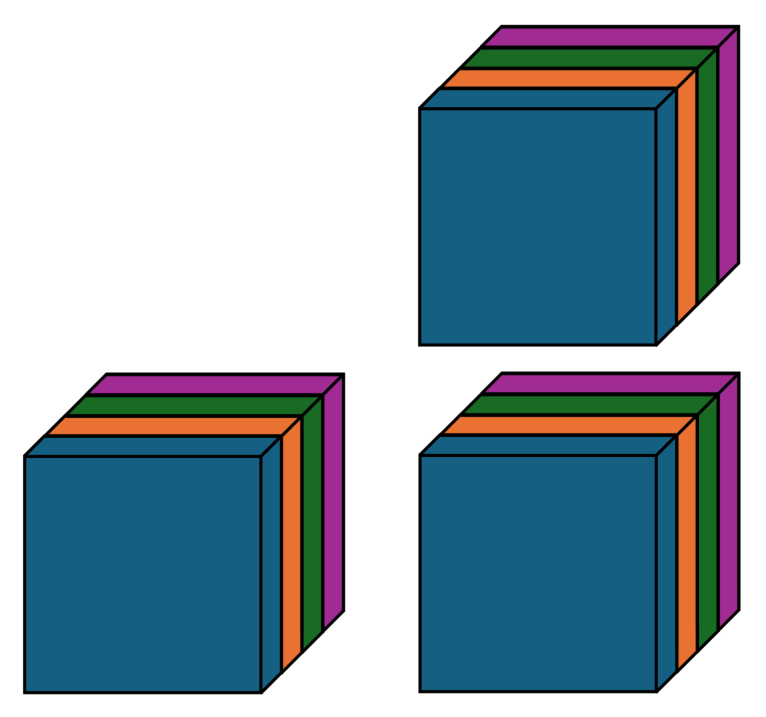
\includegraphics[width=0.3\textwidth]{dist_c.pdf} % todo : how to visualize contraction? how to show algorithm idea on n-order tensors instead of max 3
\caption{Visualization of the distributed c algorithm; 
each colour represents one node with the coloured blocks representing the data they hold; 
since the tensors are distributed along the same c dimension, each node can locally contract its chunks to generate its chunk of the output tensor.}
\label{fig:c_algo}
\end{figure}

Distribution along a c dimension is the simplest algorithm we consider. 
As seen in Figure \ref{fig:c_algo} we assume both input tensors are distributed along the same c dimension.
We also generally expect all distributions to follow the same order within ranks, meaning that rank 0 always keeps the first chunk, rank 1 the second and so on.
If now both input chunks are contracted on each node, the result will be a chunk of the output tensor distributed along the same c dimension.
This algorithm is preferable where applicable since it does not need any communication between nodes.
%todo: how to show that this is referring to n-order tensors?
%todo: how the hell do I formalize 3 tensors where a single c dimension is at any unspecified point in a contraction, that then gets split up, calculated distributed, merged and is the same?

\subsection{Distributed m/n-dimensions Algorithm}

\begin{figure}[ht]
\centering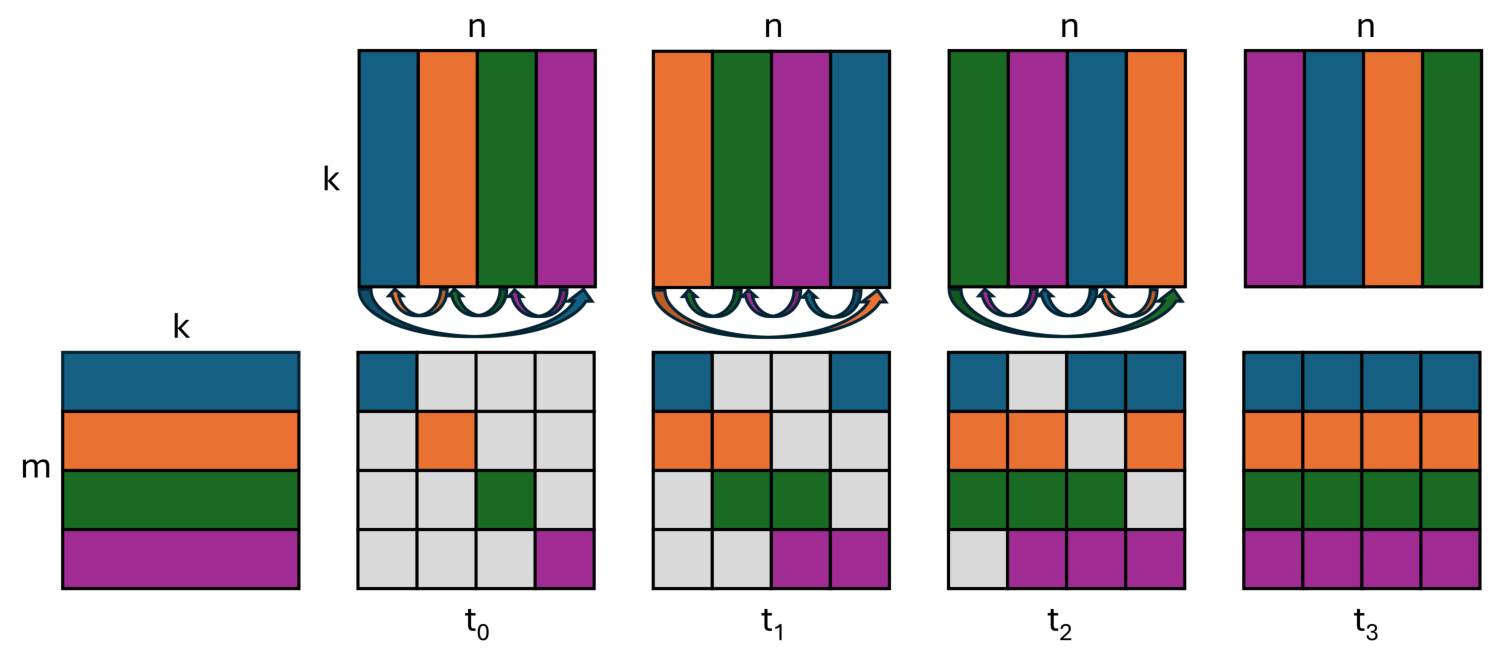
\includegraphics[width=0.75\textwidth]{dist_m_n.pdf}
\caption{Visualization of the distributed m/n algorithm for order-2 tensors; 
each colour represents one node with the coloured blocks representing the data they hold;
The arrows visualize which tensor a node, represented on the arrow colour, acquires next.
}
\label{fig:m_n_algo}
\end{figure}

\begin{figure}[ht]
\centering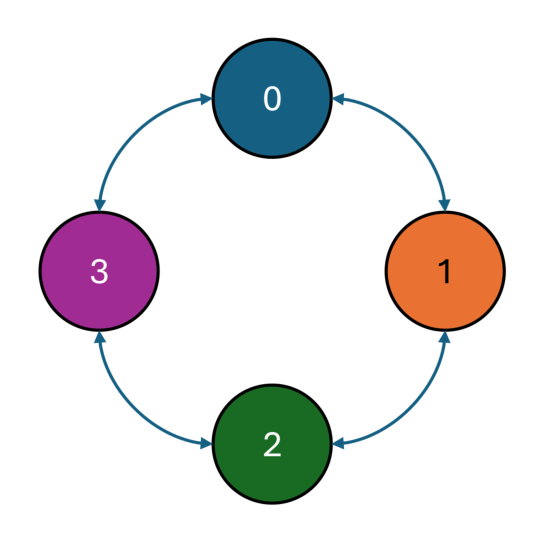
\includegraphics[width=0.2\textwidth]{ring.pdf}
\caption{Visualization of ring communication: Each node only communicates with its immediate neighbour.}
\end{figure}


For the communication of this algorithm we assume that all node are set up in a ring as seen in the right part of Figure \ref{fig:m_n_algo}.
If both input tensors are distributed alongside a m/n dimensions, communication between nodes is unavoidable. %todo: how to better describe m/n dimension
In contrast to the distributed c algorithm, each node can only calculate a $\frac{1}{totalNodes}$ big chunk of its output tensor locally. %todo: how to show that only a snippet of an output tensor can get calculated
Instead of gathering all the data needed to calculate the full chunk of the output tensor, we'll proceed in $\frac{1}{totalNodes}$ subchunks. %todo: how to introduce subchunks
Each node starts with the data to contract a single subchunk of its output tensor.
This output chunk will be offset based on the rank of each node, as shown in Figure \ref{fig:m_n_algo}.
While each node contracts its first chunk, they also each send their currently contracting right chunk towards the previous node in the ring.
To achieve that each node will use an extra communication thread so the communication gets overlapped with the contraction and allocate an extra buffer for the receiving tensor to go into.
After each step the receiving and calculating tensors switch their functions.
After $totalNodes$ iterations each node has one chunk of the output tensor that is distributed along the same dimension as the left input tensor.
While the time to communicate one chunk of the right tensor is smaller than the time to contract one subchunk, all communication times are overlapping with the computation.

Design Considerations:\\
\textbf{The implemented algorithm omits communicating tensors in the last iteration.}
This last communication is not needed since there is no contraction following.
It would only be necessary if the input tensors should finish in the same state as they started.
For trees the input tensors get deallocated directly after each contraction anyways.
In a tree each input gets only used exactly once, so the input tensors will get freed after the calculation anyways.
Should the algorithm be adjusted to also work for directed acyclic graphs, this last communication would have to occur to keep input tensors intact.
Should an uneven number of nodes be employed that last step would also need to be followed by a local copy from the allocated buffer to the original input tensor.\\
\textbf{Ring communication is chosen to reduce additional memory needed.}
If alternatively each node keeps its input tensors to send to each other node directly, it would need another two buffers, one for the chunk that is currently contracted (except in the first iteration where it already has that buffer in the form of the input tensor) and another for the tensor it currently receives.
The size of these buffers could be reduced by choosing a smaller subchunk size, but that would involve more smaller MPI packages and smaller contractions, both of which are worse for performance.
The size of the buffers in the ring algorithm could be reduced in a similar manner and still require only half of the additional memory for the same subchunk size.\\
\textbf{Due to a limitation in the current contraction interface, the distributed dimension of the right tensor has to be the outermost dimension of the output tensor.}
This is necessary since the current interface supports only the contraction of two contiguous chunks of memory into a third contiguous chunk.
To divide the output tensor into $totalNodes$ many contiguous chunks the split dimension of the subchunks needs to be the outer most dimension.
This limitation could be remedied by expanding the contraction interface to support strided input and output tensors.\\
\textbf{An algorithm for keeping the distributed dimension of the right tensor is not needed.}
This algorithm would work completely analogously to the m/n algorithm depicted but communicate the left tensor across nodes instead.
To achieve the same result the two contracted tensors may be swapped in the tree without any restriction, which achieves the same result.

%todo: write why interleaving multiple timesteps was not explored (time constraints, would help if nodes have irregular breaks for example)
%todo: where should I describe why I implement tensor parallelism instead of pipeline parallelism (not suited if tree is relatively flat) or "tree" parallelism (not suited if tree is relatively deep)
%todo: use einsum notation somewhere (?)
%todo: should I describe here why I only expect 1 dimension to be split (1 split into 4 instead of 2 into 2 each for example)

\subsection{Distributed k-dimension Algorithm}

\begin{figure}[ht]
    \centering{
    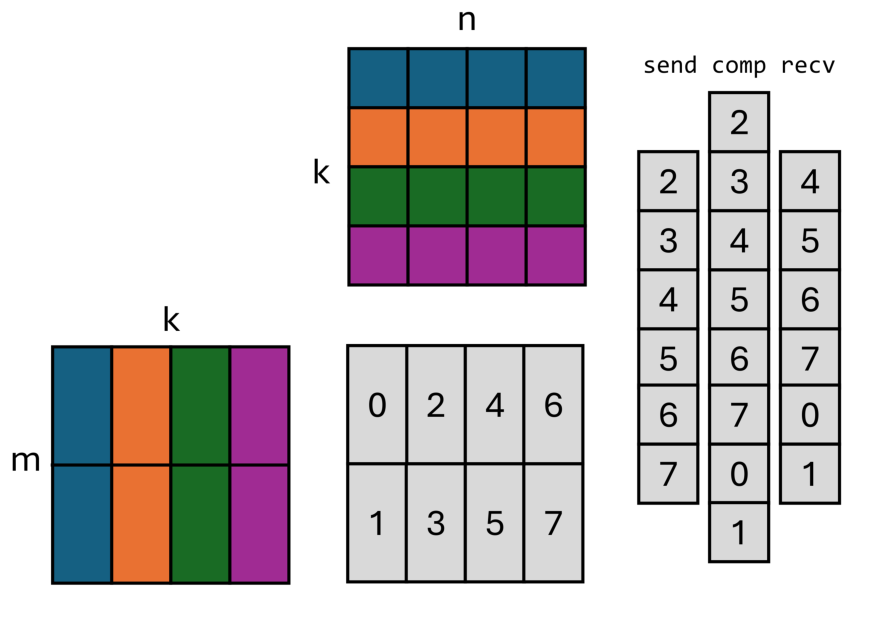
\includegraphics[width=0.5\textwidth]{dist_k.pdf}
    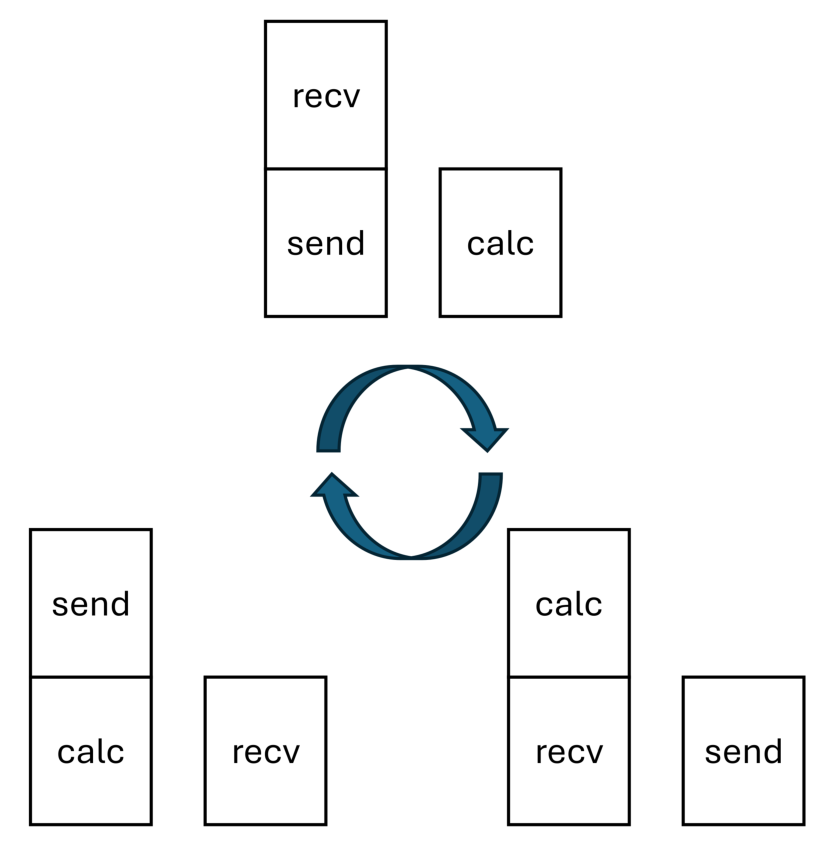
\includegraphics[width=0.34\textwidth]{dist_k_memory.pdf}
    }
    \caption{Visualization of the distributed k algorithm; 
    each colour represents one node with the coloured blocks representing the data they hold; 
    In contrast to the m/n algorithm in Figure \ref{fig:m_n_algo}, this algorithm moves the output tensor through the nodes.
    The left graphic depicts the data movement from the perspective of rank 0 for 4 nodes.
    It starts with the chunk of the next rank and then linearly adds its part of the contraction to each, ending with its own chunk of the output tensor, at which point the contraction completes.
    The right graphic depicts the memory layout used, with two contiguous chunks being stored in the output tensor and one extra chunk as additional memory.
    After each timestep the function of each tensor rotates ($calc \rightarrow send \rightarrow recv \rightarrow calc$).
    After three timesteps each tensor has the same function.
    To end with its whole chunk in the output tensor the last timestep has to use the bottom left format.
    }
    \label{fig:k_algo}
\end{figure}

For the communication of this algorithm we once again assume a ring like setup like the distributed m/n-dimension one.
We assume that both input tensors are distributed along the same k dimension and that the outer most dimension of the left tensor is the same as that of the output tensor.
In contrast to the m/n-dimension algorithm each node no longer calculates one full subchunk of the output tensor.
Instead, each node calculates a part of all output chunks with its local inputs.
So instead of communicating one of the input tensors, the nodes communicate their partial sums.
Since the k dimension is no longer in the output we can choose an arbitrary dimension to distribute the output tensor on, in Figure \ref{fig:k_algo} we split the output tensor along an n dimension.
Since each node should end up with its own corresponding output tensor chunk, they will each start contracting the chunk of their next neighbour in the ring.
Then after each contraction they will send the contracted tensor to their previous neighbour.
That way after all contractions they will each end up with their corresponding chunk.
To overlap communication and computation a tensor in this case can't be simultaneously calculated on and received or sent.
To circumvent this problem, we also split the left and output tensor along their outermost dimension in 2 parts to generate 2 subchunks.
Now in each step the second half of an output tensor chunk can be computed while the first part already gets sent.
With now in total $2 \cdot totalNodes$ chunks to calculate the algorithm takes an equal number of steps.
In each step the previous result gets sent to the previous node in the ring, while the current subchunk gets calculated and the next chunk loaded from the next node in the ring.
The only exception to that is the first and last step, where in the first step there are no tensors yet to be communicated and in the last step the results are already in the right places.
An example for all timesteps for rank 0 in a 4 node ring is depicted in Figure \ref{fig:k_algo}.

In total we need three subchunks on each node to execute the algorithm.
We use the output tensor to store two of them and allocate an additional temporary tensor for the third one.
The chunks start in either of the positions depicted on the right of Figure \ref{fig:k_algo}.
To determine the starting position the last two steps in the algorithm have to be considered.
The last step should calculate the bottom part of the output tensor (so bottom left) and the second to last step should calculate the top part of the output tensor (so bottom right).
After each step the three subchunks "rotate" functions.
The last calculated subchunk gets sent out next, the last sent subchunk is now free to receive new data and the last receive chunk now has to be contracted on.
After three iterations all subchunks have the same function.
With that in mind we can calculate the starting position of all chunks with a simple modulo calculation, since we know the end position and the number of "rotations" that happen.

A few design considerations should be noted again:\\
\textbf{Due to a limitation in the current contraction interface, the distributed dimension of the output has to be the outermost dimension of its input tensor.}
To be able to split the input tensor into subchunks to contract individually, the outer most dimension has to be split.
As with the m/n-algorithm this could be solved by supporting strided input in the interface.\\
\textbf{The distributed dimension of the output tensor may be the same as the split dimension for the subchunks, provided its the outermost dimension.}
In this case the dimension just has to be divisible by $2 \cdot totalNodes$ instead.\\
\textbf{If the outer most dimension of the output should not be split, it would take double the amount of additional memory.}
Assuming the interface supported strided input, it would still need a full output chunk of memory to store it in instead of only half a chunk it needs if the outer most dimension is split.\\
\textbf{Ring communication is chosen to reduce additional memory needed.}
If alternatively each node kept its output tensor and only send updates to each respective output tensor, wee would once again need enough additional memory to keep two such updates at the same time (one that gets calculated and one that gets sent to the respective node).
It would also need to call a reduction on the node where the update gets sent to, using more compute resources than the ring algorithm.


